\documentclass{beamer}
\mode<presentation>
\usepackage{amsmath}
\usepackage{amssymb}
%\usepackage{advdate}
\usepackage{adjustbox}
\usepackage{subcaption}
\usepackage{enumitem}
\usepackage{multicol}
\usepackage{mathtools}
\usepackage{listings}
\usepackage{url}
\def\UrlBreaks{\do\/\do-}
\usetheme{Boadilla}
\usecolortheme{lily}
\setbeamertemplate{footline}
{
  \leavevmode%
  \hbox{%
  \begin{beamercolorbox}[wd=\paperwidth,ht=2.25ex,dp=1ex,right]{author in head/foot}%
    \insertframenumber{} / \inserttotalframenumber\hspace*{2ex} 
  \end{beamercolorbox}}%
  \vskip0pt%
}
\setbeamertemplate{navigation symbols}{}

\providecommand{\nCr}[2]{\,^{#1}C_{#2}} % nCr
\providecommand{\nPr}[2]{\,^{#1}P_{#2}} % nPr
\providecommand{\mbf}{\mathbf}
\providecommand{\pr}[1]{\ensuremath{\Pr\left(#1\right)}}
\providecommand{\qfunc}[1]{\ensuremath{Q\left(#1\right)}}
\providecommand{\sbrak}[1]{\ensuremath{{}\left[#1\right]}}
\providecommand{\lsbrak}[1]{\ensuremath{{}\left[#1\right.}}
\providecommand{\rsbrak}[1]{\ensuremath{{}\left.#1\right]}}
\providecommand{\brak}[1]{\ensuremath{\left(#1\right)}}
\providecommand{\lbrak}[1]{\ensuremath{\left(#1\right.}}
\providecommand{\rbrak}[1]{\ensuremath{\left.#1\right)}}
\providecommand{\cbrak}[1]{\ensuremath{\left\{#1\right\}}}
\providecommand{\lcbrak}[1]{\ensuremath{\left\{#1\right.}}
\providecommand{\rcbrak}[1]{\ensuremath{\left.#1\right\}}}
\theoremstyle{remark}
\newtheorem{rem}{Remark}
\newcommand{\sgn}{\mathop{\mathrm{sgn}}}
\providecommand{\abs}[1]{\left\vert#1\right\vert}
\providecommand{\res}[1]{\Res\displaylimits_{#1}} 
\providecommand{\norm}[1]{\lVert#1\rVert}
\providecommand{\mtx}[1]{\mathbf{#1}}
\providecommand{\mean}[1]{E\left[ #1 \right]}
\providecommand{\fourier}{\overset{\mathcal{F}}{ \rightleftharpoons}}
%\providecommand{\hilbert}{\overset{\mathcal{H}}{ \rightleftharpoons}}
\providecommand{\system}{\overset{\mathcal{H}}{ \longleftrightarrow}}
	%\newcommand{\solution}[2]{\textbf{Solution:}{#1}}
%\newcommand{\solution}{\noindent \textbf{Solution: }}
\providecommand{\dec}[2]{\ensuremath{\overset{#1}{\underset{#2}{\gtrless}}}}
\newcommand{\myvec}[1]{\ensuremath{\begin{pmatrix}#1\end{pmatrix}}}
\let\vec\mathbf

\lstset{
%language=C,
frame=single, 
breaklines=true,
columns=fullflexible
}
\numberwithin{equation}{section}
\author{Ankit Jainar \\EE24BTECH11004\\IIT Hyderabad.}
\date{\today} 
\begin{document}

\begin{frame}
\titlepage
\end{frame}

\section*{Outline}
\begin{frame}
\tableofcontents
\end{frame}
\section{Problem}
\begin{frame}
\frametitle{Problem Statement}

Find the coordinates of the points which divide the line segment joining A(-2, 2) and B(2, 8) into four equal parts.

\end{frame}

\section{Solution}
\subsection{Section Formula}
\begin{frame}
\frametitle{Section Formula}

The section formula for internal division, the coordinates of the point dividing the line in the ratio $k:1$ are given by:

\begin{align}
R_k &= \left( \frac{k \cdot x_2  +  x_1}{k+1}, \frac{k \cdot y_2 +  y_1}{k+1} \right)
\end{align}

\end{frame}
\subsection{Ratio's}
\begin{frame}
\frametitle{Ratio's}
$k = \frac{i}{n-i}$ $n$, $0<i<n$ is number of equal parts \\
For $n = 4$ \\
now for
\begin{align}
R_1,k&=\frac{1}{3}\\
R_2,k&=1\\
R_3,k&=3
\end{align}
\end{frame}
\subsection{Point's}
\begin{frame}
\frametitle{Point's}
substituting A=\brak{-2,2} and B=\brak{2,8} in $R_k$
we get \\
\begin{align}
   R_1&=\brak{-1.0,3.5}\\
   R_2&=\brak{0.0,5.0}\\
   R_3&=\brak{1.0,6.5}
\end{align}	
\end{frame}
\subsection{Plot}
\begin{frame}
\frametitle{Plot}
\begin{figure}
    \centering
    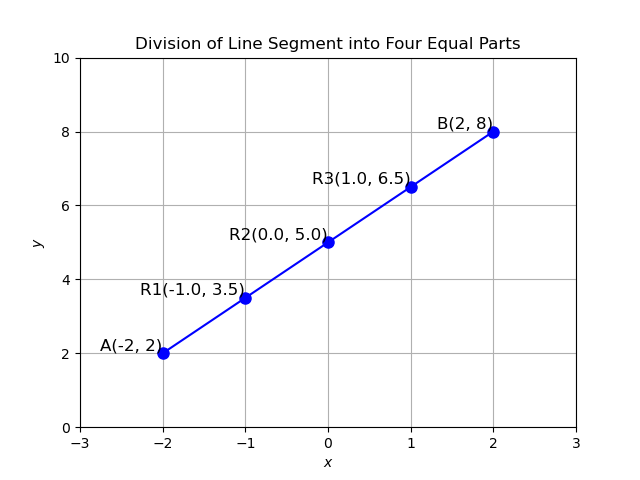
\includegraphics[width=0.5\linewidth]{figs/Figure_1.png}
    \caption{Stem Plot of y\brak{n}}
    \label{stemplot}
\end{figure}	
\end{frame}
\begin{frame}
\frametitle{C code}
\begin{figure}
    \centering
    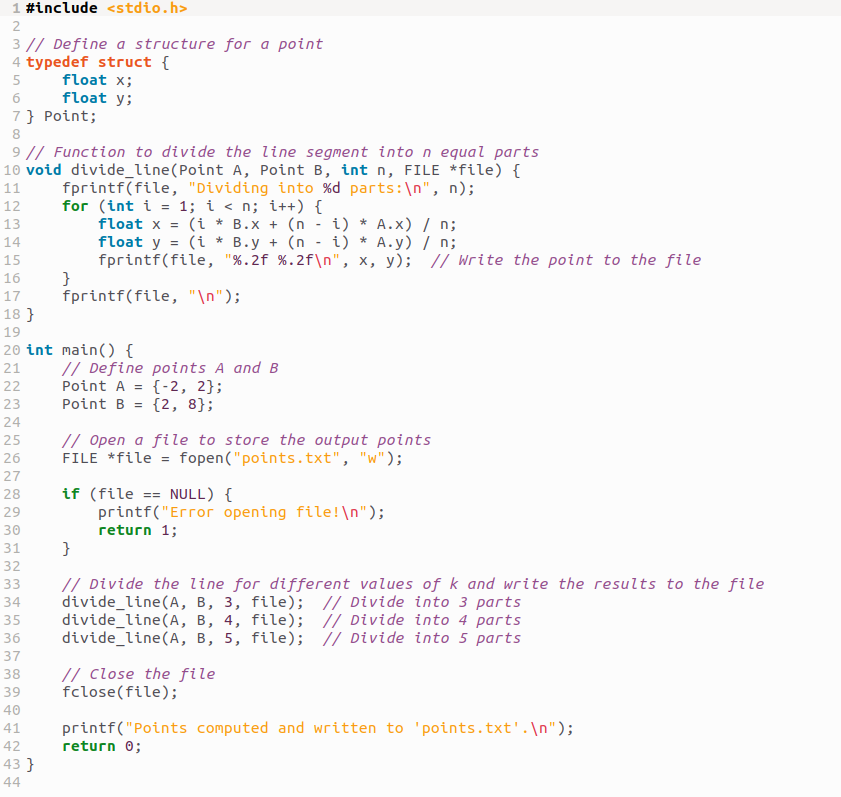
\includegraphics[width=0.5\linewidth]{figs/Figure_3.png}
   
\end{figure}	
\end{frame}
\begin{frame}
\frametitle{Python code}
\begin{figure}
    \centering
    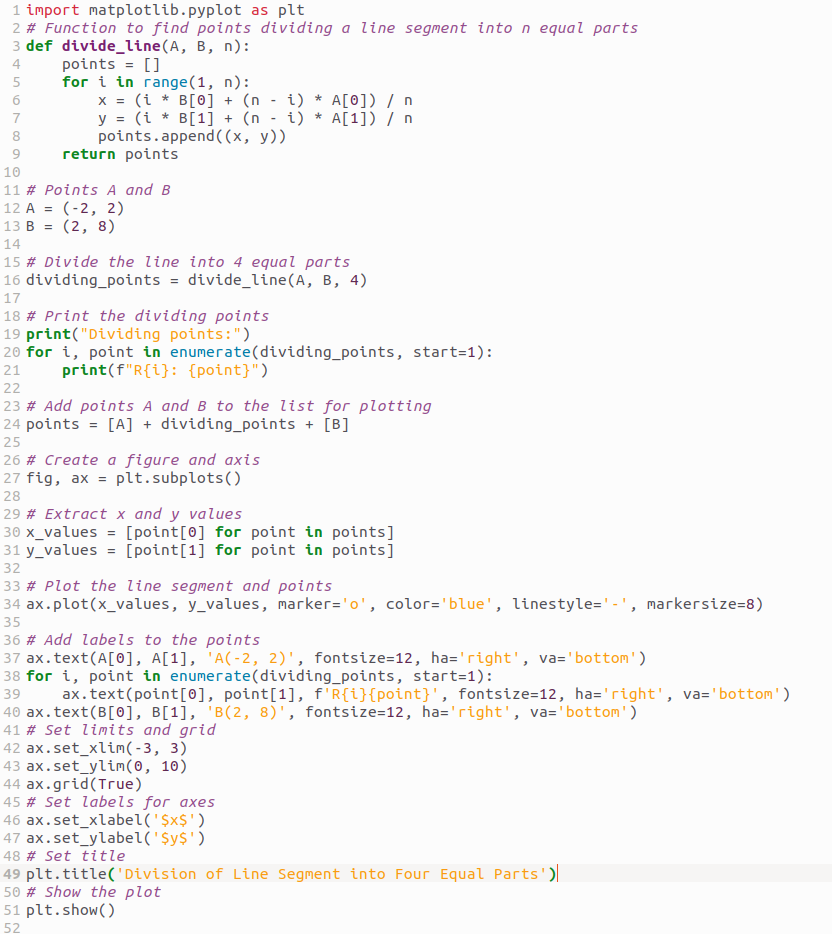
\includegraphics[width=0.5\linewidth]{figs/Figure_2.png}
    
    
\end{figure}	
\end{frame}

\end{document}\documentclass{article}
\usepackage{graphicx} 

